%\section{Função logística}


%%%%%%%%%%%%%%%%%%%%%%%%%%%%%%%%%%%%%%%%%%%%%%%%%%%%%%%%%%%%%%%%%%%%%%%%%%%%%%%%
\index{Função!Logística}
\index{Função!Sigmoide}
\begin{minipage}{0.55\textwidth}
\begin{definition}[Função sigmoid ou Função logística  $f:~\mathbb{R} \rightarrow \mathbb{R}$:]\label{def:logisticfunc}
Função $f(u)$, definida como na Eq. (\ref{eq:logisticfunc}), 
com domínio real e 
contradomínio real acotado entre 0 e 1. \cite[pp. 27]{kurkova2001artificial},
\begin{equation}\label{eq:logisticfunc}
f(u)=\frac{1}{1+e^{-u}}.
\end{equation}
A derivada da função logística cumpre a seguinte propriedade: 
\begin{equation}\label{eq:derlogisticfunc}
\frac{df(u)}{du}=f(u)(1-f(u)).
\end{equation}
\end{definition}
\end{minipage}
\begin{minipage}{0.45\textwidth}
     \begin{figure}[H]
         \centering
         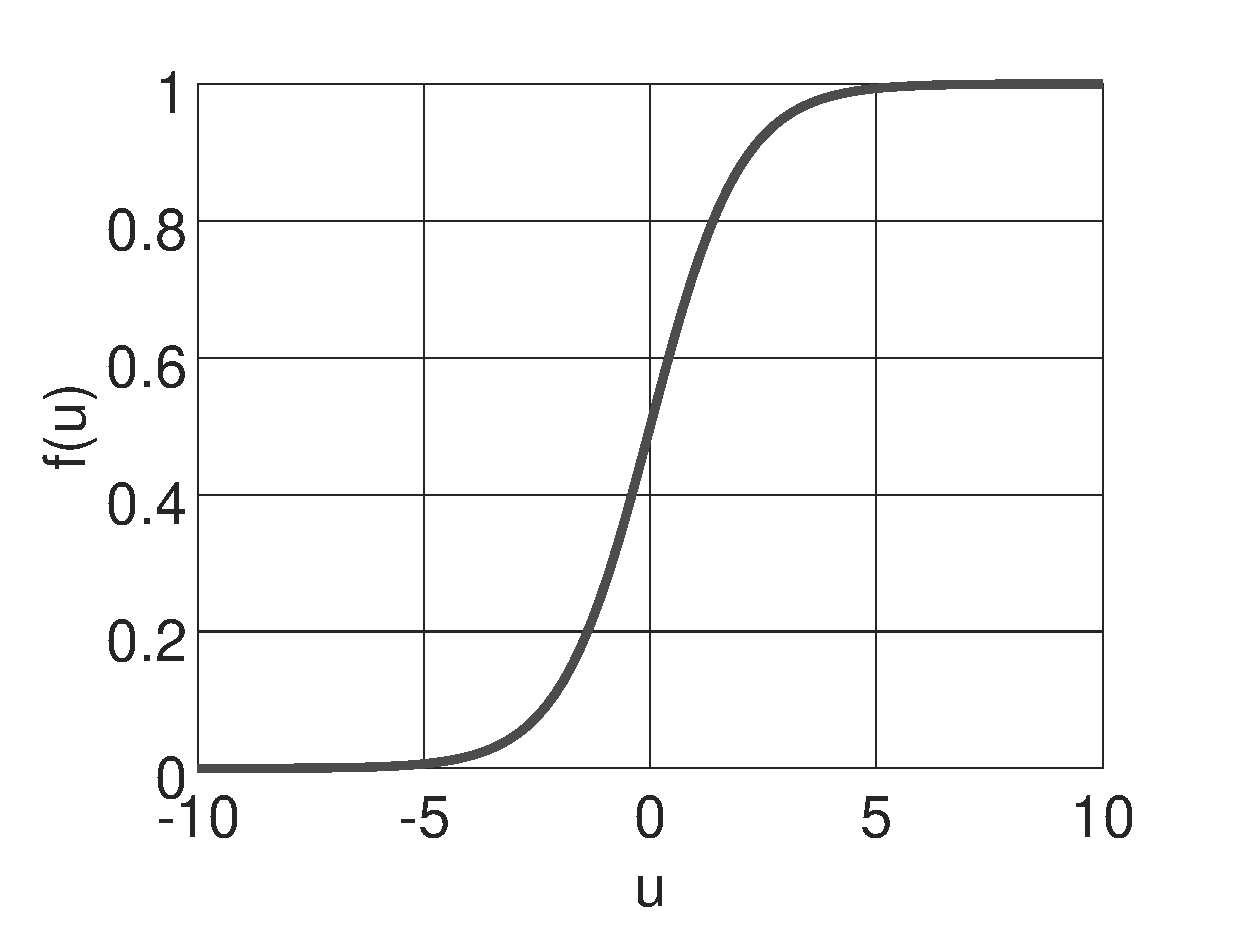
\includegraphics[width=0.9\textwidth]{chapters/classificacao/mfiles/logisticfunc/sigmoid.eps}
         \caption{Função sigmoide. }
         \label{fig:logisticfunc}
     \end{figure}
\end{minipage}
%%%%%%%%%%%%%%%%%%%%%%%%%%%%%%%%%%%%%%%%%%%%%%%%%%%%%%%%%%%%%%%%%%%%%%%%%%%%%%%%
\index{Função!Logit}
\noindent
\begin{minipage}{0.55\textwidth}
\begin{definition}[Função $logit:~\mathbb{R} \rightarrow \mathbb{R}$:]\label{def:logitfunc}
A função $logit(f)$ é definida como na Eq. (\ref{eq:logitfunc}), 
com domínio entre 0 e 1 e 
contradomínio que atinge todos os números reais. \cite[pp. 17]{kleinbaum2010logistic},
\begin{equation}\label{eq:logitfunc}
\begin{matrix}
u & = & logit(f),\\
~ & = & ln\left( \frac{f}{1-f}\right).
\end{matrix}
\end{equation}
A função logit pode ser entendida como a função inversa da função logística.
\end{definition}
\end{minipage}
\begin{minipage}{0.45\textwidth}
     \begin{figure}[H]
         \centering
         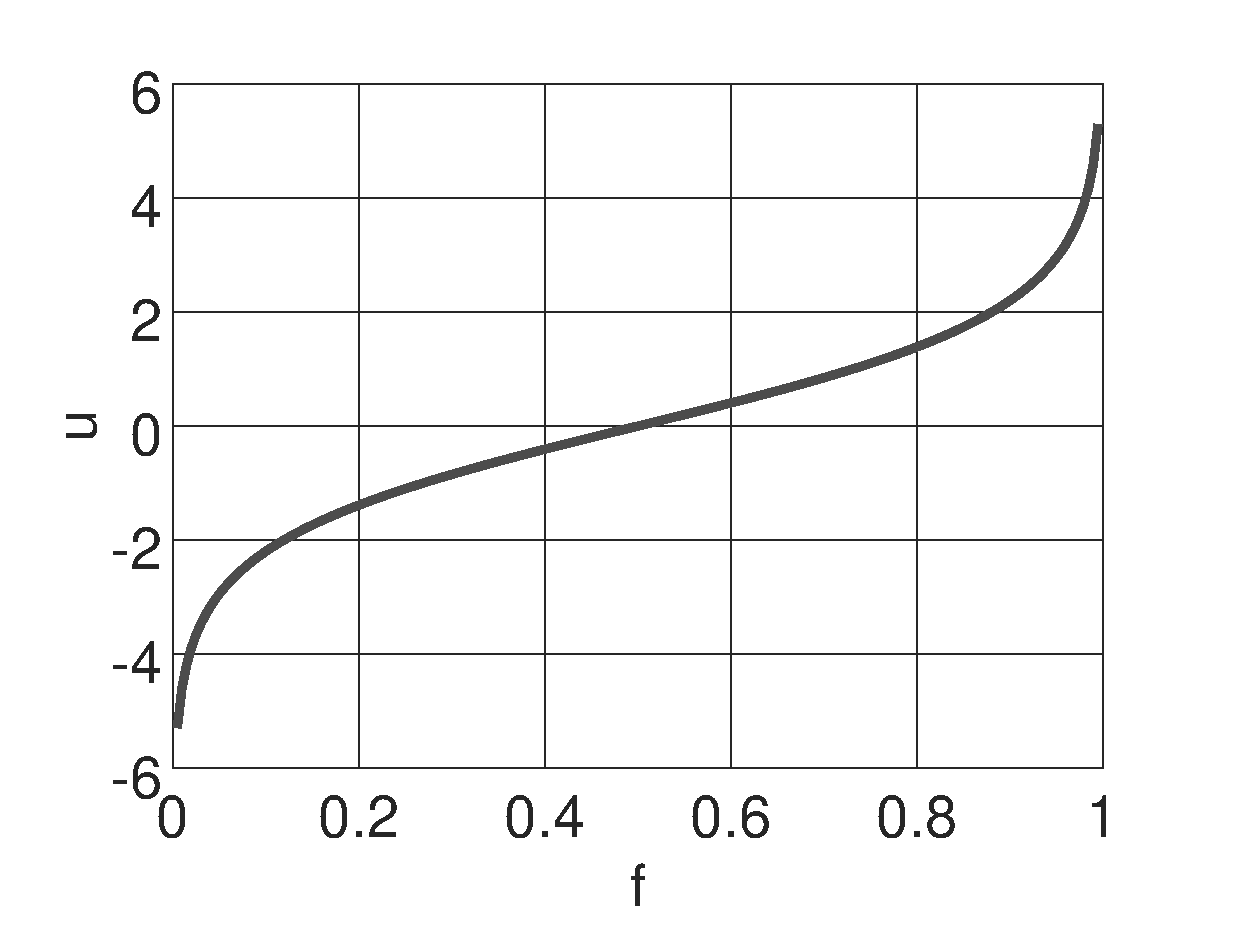
\includegraphics[width=0.9\textwidth]{chapters/classificacao/mfiles/logisticfunc/logit.eps}
         \caption{Função logit. }
         \label{fig:logitfunc}
     \end{figure}
\end{minipage}
%%%%%%%%%%%%%%%%%%%%%%%%%%%%%%%%%%%%%%%%%%%%%%%%%%%%%%%%%%%%%%%%%%%%%%%%%%%%%%%%
\begin{tcbattention}
\begin{itemize}
\item $MSE$: Sigla da frase no inglês ``mean square error'', que significa ``erro quadrático médio''.
\item $SE$: Sigla da frase no inglês ``square error'', que significa ``erro quadrático''.
\end{itemize}
\end{tcbattention}
